\documentclass[a4paper,11pt]{article}
\usepackage{amsmath,amsthm,amsfonts,amssymb,amscd,amstext,vmargin,graphics,graphicx,tabularx,multicol} 
\usepackage[francais]{babel}
\usepackage[utf8]{inputenc}  
\usepackage[T1]{fontenc} 
\usepackage{pstricks-add,tikz,tkz-tab,variations}
\usepackage[autolanguage,np]{numprint} 
\usepackage{calc}

\setmarginsrb{1.5cm}{0.5cm}{1cm}{0.5cm}{0cm}{0cm}{0cm}{0cm} %Gauche, haut, droite, haut
\newcounter{numexo}
\newcommand{\exo}[1]{\stepcounter{numexo}\noindent{\bf Exercice~\thenumexo} : }
\reversemarginpar

\newcommand{\bmul}[1]{\begin{multicols}{#1}}
\newcommand{\emul}{\end{multicols}}

\newcounter{enumtabi}
\newcounter{enumtaba}
\newcommand{\q}{\stepcounter{enumtabi} \theenumtabi.  }
\newcommand{\qa}{\stepcounter{enumtaba} (\alph{enumtaba}) }
\newcommand{\initq}{\setcounter{enumtabi}{0}}
\newcommand{\initqa}{\setcounter{enumtaba}{0}}

\newcommand{\be}{\begin{enumerate}}
\newcommand{\ee}{\end{enumerate}}
\newcommand{\bi}{\begin{itemize}}
\newcommand{\ei}{\end{itemize}}
\newcommand{\bp}{\begin{pspicture*}}
\newcommand{\ep}{\end{pspicture*}}
\newcommand{\bt}{\begin{tabular}}
\newcommand{\et}{\end{tabular}}
\renewcommand{\tabularxcolumn}[1]{>{\centering}m{#1}} %(colonne m{} centrée, au lieu de p par défault) 
\newcommand{\tnl}{\tabularnewline}

\newcommand{\trait}{\noindent \rule{\linewidth}{0.2mm}}
\newcommand{\hs}[1]{\hspace{#1}}
\newcommand{\vs}[1]{\vspace{#1}}

\newcommand{\N}{\mathbb{N}}
\newcommand{\Z}{\mathbb{Z}}
\newcommand{\R}{\mathbb{R}}
\newcommand{\C}{\mathbb{C}}
\newcommand{\Dcal}{\mathcal{D}}
\newcommand{\Ccal}{\mathcal{C}}
\newcommand{\mc}{\mathcal}

\newcommand{\vect}[1]{\overrightarrow{#1}}
\newcommand{\ds}{\displaystyle}
\newcommand{\eq}{\quad \Leftrightarrow \quad}
\newcommand{\vecti}{\vec{\imath}}
\newcommand{\vectj}{\vec{\jmath}}
\newcommand{\Oij}{(O;\vec{\imath}, \vec{\jmath})}
\newcommand{\OIJ}{(O;I,J)}


\newcommand{\reponse}[1][1]{%
\multido{}{#1}{\makebox[\linewidth]{\rule[0pt]{0pt}{20pt}\dotfill}
}}

\newcommand{\titre}[5] 
% #1: titre #2: haut gauche #3: bas gauche #4: haut droite #5: bas droite
{
\noindent #2 \hfill #4 \\
#3 \hfill #5

\vspace{-1.6cm}

\begin{center}\rule{6cm}{0.5mm}\end{center}
\vspace{0.2cm}
\begin{center}{\large{\textbf{#1}}}\end{center}
\begin{center}\rule{6cm}{0.5mm}\end{center}
}



\begin{document}
\pagestyle{empty}
\titre{Séance d'AP 4 : Notions de vitesse}{}{}{3ème}{}

\vspace*{0.2cm}

\setlength{\fboxrule}{2pt}
\begin{flushleft}
\framebox{\begin{minipage}{\linewidth}

\vspace*{0.2cm}

\underline{\textbf{{\large Rappels de cours}}}\\

La \textbf{vitesse moyenne} d'un mobile $v$ est le quotient de la \textbf{distance} parcourue $d$ par la \textbf{durée} $t$ de ce parcours.\\

\hspace*{5cm} $v=\dfrac{d}{t}$ \hspace*{1cm}ou \hspace*{0.3cm} $d=v \times t$ \hspace*{1cm} ou \hspace*{0.3cm} $t=\dfrac{d}{v}$\\

Si la distance $d$ est en kilomètres et la durée $t$ est en heures alors la vitesse s'exprime en kilomètres par heures, noté $km/h$ ou $km.h^{-1}$ \\

Il faut toujours que les unités concordent donc des conversions sont parfois utiles.\\


\end{minipage}}
\end{flushleft}

\vspace*{0.4cm}



{\large \textbf{PARTIE 1 :}\textbf{ Application des formules}}\\

\vspace{0.5cm}
Vous choisirez pour cette première partie, \textbf{3 questions} du niveau que vous souhaitez.\\

\vspace{0.5cm}

\textbf{\underline{Niveau débutant}}

1) Florent Manaudou nage 50 m en 20 s. Calculer sa vitesse en m/s.\\

2) Un escargot glisse à 2 cm/s. Combien de temps met-il pour parcourir 160 mm ? \\

3) Ophélie a parcouru 60 km à la vitesse de 40 km/h. Quelle est la durée du trajet? \\



\textbf{\underline{Niveau confirmé}}

1) Un athlète fait 82 tours de 4.2 km en 1 heure et demie. Quelle est sa vitesse moyenne ? \\

2) Un avion de ligne vole à 900 km/h pendant 2 h 20 mn. Quelle est la distance parcourue ? \\

3) En combien de temps (en secondes), un scooter parcourt-il 500 m à la vitesse de 22 km/h ?\\

\textbf{\underline{Niveau expert}}

1) Le grondement du tonnerre met 5 s à nous parvenir.
Calculer la distance qui me sépare de l'orage (vitesse du son = 330 m/s).\\

2) Calculer le temps mis par la lumière venant de cet orage pour arriver jusqu'à nous. (vitesse de la lumière = 300 000 km/s)\\

3) Le voyage sur Mars mettra 6 mois pour une distance de 500 millions km. Calculer la vitesse moyenne du vaisseau spatial.\\

\vspace{0.5cm}


{\large \textbf{PARTIE 2 :}\textbf{ Des problèmes autour de la vitesse moyenne}}\\

\vspace{0.5cm}

\exo \\

L'explosion d'un volcan, situé en mer, provoque la formation d'un raz de marée ou « tsunami » : vague de plusieurs dizaines de mètres
de hauteur se déplaçant à la vitesse de 138,89 m/s.\\

\initq
\noindent \q Transformer cette vitesse pour l'obtenir en m/h puis en km/h.\\
\q En combien de temps la vague va t-elle atteindre la maison ?\\


\vspace*{0.5cm}
\noindent \q Quelle distance aura parcouru la vague en 1 s, puis en 1 min puis en 45 min ?\\
\q En supposant que la vague mette 18 min pour atteindre le rivage, à quelle distance de celui-ci le volcan est-il situé ?\\

\begin{center}
\includegraphics[scale=0.9]{vitesse2.eps} 
\end{center}

\vspace*{0.3cm}

\exo \\
Nina est aux Estables pour une « sortie-ski » avec sa classe. Elle est au pied du TELESKI CHALET 2 où personne n'attend. Il est 16 h 50 et son professeur a donné rendez-vous au pied des pistes à 17 h précises pour le retour. \\
Nina descend en moyenne à 15 km/h. \\
A-t-elle le temps de faire une dernière descente ?\\


\begin{center}
\includegraphics[scale=0.65]{vitesse3.eps} 
\end{center}

La réponse sera donnée sous forme d'un texte présentant la démarche et les arguments.\\

\vspace*{0.3cm}

\exo \\

Le n\oe{ud} est un unité de vitesse utilisée en navigation et valant 1,852 km/h.\\
Dans la suite de l'exercice, on arrondira les résultats à l'unité.\\

\noindent \initq \q \initqa  \qa Un navire A se déplace à la vitesse moyenne de 35 n\oe{uds}. Quelle est sa vitesse moyenne en km/h ?\\
\qa À cette vitesse quelle distance parcourt-il en 1 h 30 min ?\\
\q Un navire B se déplace à la vitesse moyenne de 20 n\oe{uds}. Combien de temps lui faudra-t-il pour rejoindre un port situé à 74 km ?\\

\vspace*{0.3cm}


\exo \\
ÉNIGME

Une voiture roule la moitié d'un trajet à 80 km/h et l'autre moitié à 20 km/h.\\
Quelle est la vitesse moyenne sur le trajet entier ?\\


\end{document}
